\hypertarget{ux8ba1ux7b97ux6027ux80fdux4e0eai-infra}{%
\chapter{计算性能与AI-Infra}\label{ux8ba1ux7b97ux6027ux80fdux4e0eai-infra}}

\hypertarget{ux786cux4ef6ux90e8ux4ef6}{%
\section{硬件部件}\label{ux786cux4ef6ux90e8ux4ef6}}

\hypertarget{ux4e00ux8ba1ux7b97ux673aux7684ux57faux672cux7ec4ux6210}{%
\subsection{一、计算机的基本组成}\label{ux4e00ux8ba1ux7b97ux673aux7684ux57faux672cux7ec4ux6210}}

计算机由中央处理器（CPU）、内存（RAM）、固态存储器（外存）、图形处理器（GPU）、网络等部件组成。内存直接连接到CPU，外存和GPU通过高速扩展总线（PCIe）与中央处理器相连。为了提升性能，我们不希望系统中的任何一个部分成为瓶颈，计算和通信的速度都需要提升。

\hypertarget{ux4e8cux5185ux5b58}{%
\subsection{二、内存}\label{ux4e8cux5185ux5b58}}

内存是CPU/GPU与数据打交道的``工作台''。内存带宽很重要，但访问模式更重要。内存的访问模式有两种：随机读取和突发模式。前者意味着总是跳跃着读取内存（随机访问），后者则在一次寻址后读取一个批量的数据。

存在的瓶颈：内存虽然带宽看似很高（40-100 GB/s），但那是基于理想情况的。发送读取请求（寻址）需要100ns，而传输数据只需0.2ns。这意味着，发起一次读取请求的时间成本是传输数据的500倍。

性能优化策略：避免随机读取，尽量使用突发模式。这解释了为什么深度学习中张量通常是连续存储的，以及为什么批量处理如此重要。同时，数据结构应与硬件的物理存储体边界对齐。

GPU内存（GDDR6/HBM）类似于CPU内存，但为了喂饱成千上万个计算核心，它的带宽通常宽得多（位宽更大），但代价是容量小且极其昂贵。

\hypertarget{ux4e09ux5b58ux50a8ux5668}{%
\subsection{三、存储器}\label{ux4e09ux5b58ux50a8ux5668}}

\begin{enumerate}
\def\labelenumi{\arabic{enumi}.}
\item
  机械硬盘：依赖机械旋转和磁头移动，导致极高的延迟（毫秒级）和很低的吞吐量（100 IOPs）。仅适合归档，绝对不适合直接用于训练深度学习模型的数据读取，否则GPU会一直等待硬盘，造成严重的计算资源浪费。
\item
  固态硬盘：无机械结构，IOPs 提升了3个数量级，带宽提升1个数量级。由于NAND Flash的特性（必须先擦除块才能写入），随机写入性能较差。传统SATA接口太慢，NVMe协议通过PCIe通道直接连接CPU，解除了带宽封印（可达8GB/s），是目前高性能AI服务器的标配。
\item
  云存储：灵活性强，用户可以根据训练任务（是大文件还是大量小文件）动态调整IOPs。
\end{enumerate}

\hypertarget{ux56dbcpu}{%
\subsection{四、CPU}\label{ux56dbcpu}}

虽然深度学习主要靠GPU，但CPU仍然负责逻辑流控制、指令解码、以及数据预处理。CPU往往有多个核心。

\begin{enumerate}
\def\labelenumi{\arabic{enumi}.}
\tightlist
\item
  缓存（Cache）机制：内存的速度比CPU慢了约200-500倍，如果没有缓存，CPU每执行一条指令都要等内存几百个周期。故我们采用缓存机制。
\end{enumerate}

缓存机制之所以能减少内存读写，是因为它在``预判''接下来可能用到什么数据，提前将其存起来。这利用了时间局部性和空间局部性。前者指的是，如果你刚刚访问了某个数据，那么你很可能马上又要访问它，如for循环中的计数器变量i，刚用过的数据会被保留在L1缓存中，以备再次使用。后者指的是，如果你访问了地址X的数据，那么你很可能马上要访问地址X+1的数据，如读取Array{[}0{]}时，CPU一次性``突发读取''64个值到Array{[}63{]}，这就叫一个缓存行。接着读Array{[}1{]}时，就是``瞬间''完成的。因此，我们希望内存中紧密排列的元素也是先后要被用到的，而不是无关的（无关的反而可能带来麻烦，后面会提到）。

现代CPU采用金字塔式的缓存结构：

\begin{longtable}[]{@{}
  >{\raggedright\arraybackslash}p{(\columnwidth - 8\tabcolsep) * \real{0.20}}
  >{\raggedright\arraybackslash}p{(\columnwidth - 8\tabcolsep) * \real{0.20}}
  >{\raggedright\arraybackslash}p{(\columnwidth - 8\tabcolsep) * \real{0.20}}
  >{\raggedright\arraybackslash}p{(\columnwidth - 8\tabcolsep) * \real{0.20}}
  >{\raggedright\arraybackslash}p{(\columnwidth - 8\tabcolsep) * \real{0.20}}@{}}
\toprule
层级 & 位置 & 大小（典型值） & 速度（延迟） & 特性 \\
\midrule
\endhead
寄存器（Registers） & CPU核心内部 & 几百字节 & 0 延迟 & 实际上不是缓存，是CPU的``手''。数据必须在这里才能被计算。 \\
L1 缓存（一级） & 紧贴核心 & 32KB - 64KB & \textasciitilde1 ns（3-4 个周期） & 最快但最小。通常分为两部分：L1d（存数据）和 L1i（存指令）。每个核心独享。 \\
L2 缓存（二级） & 核心附近 & 256KB - 2MB & \textasciitilde3-10 ns & 比 L1 大，比 L1 慢。通常也是每个核心独享（或两个核心共享）。 \\
L3 缓存（三级） & 芯片共享区 & 4MB - 256MB+ & \textasciitilde10-20 ns & 所有核心共享。如果 L1/L2 没找到，就来这里找。如果还没找到，才去读内存。 \\
主内存（RAM） & 独立插槽级 & 16GB - TB & \textasciitilde100 ns & 最后的防线。 \\
\bottomrule
\end{longtable}

缓存一致性协议：确保在一个多核系统中，无论哪个核心修改了数据，其他核心都能立即``感知''到，保证大家读到的数据永远是最新的。例如主内存里有变量X = 0，A、B各自把X读入自己的L1缓存。A在自己的缓存里把X改成了1。此时主内存和核心B 的缓存里还是X = 0，如果核心B现在拿旧的X计算，程序逻辑就会出错。故当核心A修改数据时，必须通知核心B``你的数据过时了，别用了''。

性能陷阱：假设核心A在修改变量X，核心B在修改变量Y，逻辑上它们互不相干，但物理内存中它们处于同一个 64字节的缓存行中。核心A修改X，根据缓存一致性协议，核心B缓存里的这行数据（包含Y）被迫失效。核心B要写Y，发现缓存失效，必须强制从内存重新加载数据。核心B一写，又导致核心A的缓存失效。两个核心来回争夺这个缓存行的控制权，导致性能比单核还慢。解决方案：编程时通过内存对齐（Padding），强行把X和Y分开到不同的缓存行。（但不能滥用Padding，会让效率降低到内存随机读写的效率，只有满足多线程+需要高频写入+物理内存靠近，才能这么做）

\begin{enumerate}
\def\labelenumi{\arabic{enumi}.}
\setcounter{enumi}{1}
\tightlist
\item
  矢量化：CPU提速的关键。AVX2/NEON指令集允许CPU在一个时钟周期内对一组数据（如128位）同时进行操作。虽然CPU有矢量化能力，但仍远不如GPU成千上万个核心的并行能力。
\end{enumerate}

\hypertarget{ux4e94gpu}{%
\subsection{五、GPU}\label{ux4e94gpu}}

\begin{enumerate}
\def\labelenumi{\arabic{enumi}.}
\tightlist
\item
  为何神经网络训练使用GPU而非CPU？
\end{enumerate}

神经网络训练更适合使用GPU，主要是因为GPU的大规模并行架构、高内存带宽和专用计算单元能够极大提升深度学习训练的效率。两者的关键差异如下：

\begin{itemize}
\tightlist
\item
  核心架构：CPU 由少量高性能核心组成，擅长处理复杂逻辑和串行任务；GPU 拥有数千个小型计算核心，专为大规模并行计算设计。深度学习中的矩阵乘法、卷积等运算可被分解为大量相同任务，由 GPU 上千核心同时处理。
\item
  内存带宽：CPU 依赖 DDR 内存，带宽相对较低，通常是几十 GB/s；GPU 采用 HBM 等高带宽内存，带宽可达数百 GB/s 至数 TB/s，通常是 CPU 的 10 倍以上。这能快速喂食海量训练数据给计算核心，避免``数据饥饿''，极大提升吞吐量。
\item
  计算单元：CPU 使用通用计算单元；GPU 集成 Tensor Core 等专用单元，为低精度矩阵运算深度优化。因此，GPU 更适合混合精度训练，在保持模型精度的同时进一步提升计算速度和效率。
\item
  能效比：CPU 在执行大规模并行任务时能效相对较低；GPU 每瓦特性能更高，在处理相同 AI 训练任务时更具成本效益。
\end{itemize}

本质上，CPU和GPU的架构差异根植于它们不同的设计目标。CPU的目标是强大的通用性和低延迟，能高效处理操作系统、办公软件、数据库等各种各样的串行任务，保证计算机的快速响应。它像一位知识渊博的教授，能解决各种复杂问题，但一次只能专注于一个。GPU最初为图形渲染（数百万像素的并行计算）而生，其设计目标就是高吞吐量，擅长在短时间内完成海量简单的重复性计算，但不适合处理if-else等复杂逻辑。它就像一个流水线工厂，拥有成千上万的工人（核心），虽然每个工人只做简单工作，但协同合作下能高效完成大规模生产。深度学习训练主要是大量线性矩阵、激活函数、梯度的计算，正好符合``海量简单重复计算''的特性，因此与GPU的架构优势完美契合。

GPU非常讨厌稀疏数据（不连续的数据）和中断。处理图神经网络（GNN）等稀疏结构时，往往不能发挥GPU的最大性能。

\begin{enumerate}
\def\labelenumi{\arabic{enumi}.}
\setcounter{enumi}{1}
\tightlist
\item
  GPU结构与瓶颈
\end{enumerate}

GPU由计算核心（包括其中的寄存器）、HBM（显存）及二者之间的L1、L2缓存等组成。计算时，每次从显存搬运大量数据到L2缓存，从中取一小部分数据进入L1缓存，再从中取更小一部分进入计算核心的寄存器。每次当计算核心计算完毕，就回传数据，并从L1缓存中继续取数据；L1缓存取完时，就从L2缓存新加载一小批进入L1缓存；L2缓存取完时，就从显存加载一大批进入L2缓存。这样就形成了分层结构，越内层存储量越少，更新越快。

在LLM推理中，预填充阶段模型会并行处理所有输入 Token，矩阵乘法算术密度高，瓶颈主要在于算力。而自回归生成阶段，由于计算核心存储量有限，需要将模型权重从显存分批搬运到计算核心进行计算，每一批权重算完就要换成下一批权重，每生成一个token都要完成搬运一轮整个模型的权重。由于计算速度远快于显存带宽传输数据的速度，事实上GPU绝大多数时间都在等数据从显存传过来，算力利用率极低。

为什么计算核心和显存不能实现存算一体？这是因为计算核心的寄存器和旁边的L1/L2缓存使用的是SRAM（静态随机存取存储器），速度极快，但体积巨大，存储1 bit的数据需要6个晶体管，如果在这里存储，意味着一个几十B的模型也需要以平方米为单位面积的芯片。显存使用的是DRAM（动态随机存取存储器），体积极小，存储1 bit只需要1个晶体管和1个电容，但速度慢，利用1个晶体管+1个电容来存储电荷，由于电容的充放电需要时间，读取数据速度极慢，且为了保证数据不丢失，DRAM 每隔几十毫秒就必须把所有数据读出来重写一遍（刷新），当计算核心急需数据时，DRAM可能正在忙着``自我刷新''，这种不确定性对于追求极致确定性的逻辑电路来说是灾难性的。

上述问题的根源在于，逻辑工艺（Logic Process）和存储工艺（Memory Process）是两条完全不同的进化树。GPU/CPU核心（逻辑工艺）追求的是开关速度。晶体管要越快越好，漏电控制要好；DRAM（存储工艺）追求的是存储密度，在极小的空间里造出大容量电容。

\begin{enumerate}
\def\labelenumi{\arabic{enumi}.}
\setcounter{enumi}{2}
\tightlist
\item
  训练和推理的区别
\end{enumerate}

训练需要高精度（FP32/FP16混合），需要极大的显存来存储中间梯度，对应硬件如 NVIDIA V100/A100；推理只需要前向传播，不需要存梯度，精度要求低（INT8即可）。

\hypertarget{ux516dux6570ux636eux4f20ux8f93}{%
\subsection{六、数据传输}\label{ux516dux6570ux636eux4f20ux8f93}}

\begin{enumerate}
\def\labelenumi{\arabic{enumi}.}
\tightlist
\item
  数据传输通道的类型
\end{enumerate}

PCIe：系统内部的主干道。CPU与GPU、SSD之间都靠它连接。但通道数有限。如果你的CPU只有40个通道，插了4张GPU（通常每张需要16x），带宽就会受限，或者需要昂贵的Switch芯片。

NVLink：专门用于GPU之间的高速互连。带宽（300 Gbit/s）远超PCIe。在模型并行训练中，GPU之间需要频繁交换参数，如果没有NVLink，PCIe会成为严重的瓶颈，导致多卡加速比极低。

\begin{enumerate}
\def\labelenumi{\arabic{enumi}.}
\setcounter{enumi}{1}
\tightlist
\item
  如何解决数据传输瓶颈？
\end{enumerate}

（1）减少拷贝次数：在设备（CPU、GPU和其他机器）之间传输数据比计算慢得多，我们必须等待数据被发送（或者接收），因此我们需要尽量减少拷贝。

（2）集中执行操作：多个小操作比一个大操作糟糕得多，一次执行几个操作比代码中散布的许多单个操作要好得多。

（3）避免过多格式转换：当我们打印张量或将张量转换为NumPy格式时，如果数据不在内存中，框架会首先将其复制到内存中，这会导致额外的传输开销，有时也可能成为瓶颈。

\hypertarget{ux53c2ux8003ux6587ux732e-32}{%
\subsection{参考文献}\label{ux53c2ux8003ux6587ux732e-32}}

\begin{itemize}
\tightlist
\item
  Aston Zhang, Zachary C. Lipton, Mu Li, Alexander J. Smola. (2023). \href{https://zh.d2l.ai/}{《动手学深度学习》}. Cambridge University Press.
\end{itemize}

\clearpage

\hypertarget{ux6df1ux5ea6ux5b66ux4e60ux6846ux67b6}{%
\section{深度学习框架}\label{ux6df1ux5ea6ux5b66ux4e60ux6846ux67b6}}

\hypertarget{ux4e00ux547dux4ee4ux5f0fux7f16ux7a0bux4e0eux7b26ux53f7ux5f0fux7f16ux7a0b}{%
\subsection{一、命令式编程与符号式编程}\label{ux4e00ux547dux4ee4ux5f0fux7f16ux7a0bux4e0eux7b26ux53f7ux5f0fux7f16ux7a0b}}

\begin{enumerate}
\def\labelenumi{\arabic{enumi}.}
\tightlist
\item
  命令式编程
\end{enumerate}

（1）核心逻辑

``所见即所得''，代码运行到哪一行，计算机就执行哪一行，并立刻计算出结果。Python的例子：

e = add(a, b) \# 解释器立即计算 a+b，将结果存入内存 e

f = add(c, d) \# 解释器立即计算 c+d，将结果存入内存 f

（2）优点

灵活性高：可以使用Python的控制流（if, for）随意改变计算逻辑。

易于调试：程序报错时，你可以确切知道是哪一行数据出了问题，因为中间变量都保留在内存中。

（3）缺点（性能瓶颈）

Python开销大：每次操作都需要Python解释器参与，对于GPU这种极快的硬件，Python解释器可能跟不上，导致GPU空转等待。

缺乏全局优化：因为是逐行执行，系统不知道下一行要干什么，无法进行合并计算或内存复用。例如，系统必须保留 e 和 f 直到函数结束，因为它不知道后面会不会再用到它们。

\begin{enumerate}
\def\labelenumi{\arabic{enumi}.}
\setcounter{enumi}{1}
\tightlist
\item
  符号式编程
\end{enumerate}

（1）核心逻辑

``先画蓝图，再施工''，先用代码描述清楚所有的计算步骤，生成一个流程图。此时并没有真正发生计算。编译器优化这个图（例如，发现 (1+2)+(3+4) 可以直接优化为 10，或者发现某个变量用完就可以立刻释放内存），再将数据输入编译好的程序中运行。我们用一段C++代码来模拟这个过程（虽然C++属于命令式编程，但它是编译型语言，它在``执行前先进行一次编译优化''这一点上，与符号式编程的优越性有相似之处）：

\begin{verbatim}
int main() {
    // --- 阶段 1：定义过程（Symbolic Definition）---
    // 此时根本没有发生任何数学运算，只有“字符串”被记录下来

    std::vector<Node> computation_graph;

    // 定义：e = add(a, b)
    computation_graph.push_back({"e", "ADD", {"a", "b"}});

    // 定义：f = add(c, d)
    computation_graph.push_back({"f", "ADD", {"c", "d"}});

    // 定义：g = mult(e, f)
    computation_graph.push_back({"g", "MULT", {"e", "f"}});

    std::cout << ">>> 图纸绘制完毕，此时没有进行任何计算。" << std::endl;

    // --- 阶段 2：编译/优化（Compilation/Optimization）---
    // 这是符号式编程的杀手锏。
    // 编译器看到完整图纸后，发现了一个惊人的优化机会！

    std::cout << ">>> 正在编译和优化..." << std::endl;
    // 假设输入是常数：a=1, b=2, c=3, d=4
    // 编译器发现：所有的输入都是固定的！
    // 它可以直接把 (1+2)*(3+4) 优化成 21，完全删掉中间步骤。

    // 优化后的图纸可能只剩下一条指令：
    std::string optimized_instruction = "Return 21";

    // --- 阶段 3：执行（Execution）---
    std::cout << ">>> 开始执行:" << std::endl;
    std::cout << optimized_instruction << std::endl;
}
\end{verbatim}

（2）优点

效率极高：编译器可以看到全局视图，进行内存优化、算子融合。

可移植性：一旦编译成计算图，就不再依赖Python环境，可以将模型及其参数序列化（保存）到磁盘，在运行时直接根据计算图进行计算即可。这允许这些训练好的模型部署到其他设备（如移动端）上，并且还能方便地使用C++等其他前端编程语言。

（3）缺点

调试困难：因为定义和执行是分离的，报错往往很难定位到最初的Python代码行。

学习曲线陡峭：不如Python直观。

\begin{enumerate}
\def\labelenumi{\arabic{enumi}.}
\setcounter{enumi}{2}
\tightlist
\item
  混合式编程
\end{enumerate}

早期的深度学习框架往往是命令式编程与符号式编程中的一个，如Theano、TensorFlow、Keras和CNTK采用了符号式编程。相反地，Chainer和PyTorch采取了命令式编程。在后来的版本更新中，TensorFlow2.0和Keras增加了命令式编程。

随着人工智能的发展，算力需求越来越大，多GPU并行处理成为常态，此时单线程的Python解释器无疑会成为瓶颈。为了能实现符号式编程的效率和可移植性，又保留命令式编程的可开发性，混合式编程应运而生。它将这两种编程模型的优点结合起来，如torchscript，让用户能用命令式编程进行开发和调试，同时能够将大多数程序转换为符号式程序，以便在需要产品级计算性能和部署时使用。例如，我们定义了一个MLP网络net，用net = torch.jit.script(net)就可以转换为可编译和优化的模式。

\hypertarget{ux4e8cux5f02ux6b65ux8ba1ux7b97}{%
\subsection{二、异步计算}\label{ux4e8cux5f02ux6b65ux8ba1ux7b97}}

\begin{enumerate}
\def\labelenumi{\arabic{enumi}.}
\tightlist
\item
  异步计算的核心思想
\end{enumerate}

（1）Python（服务员）收到指令b = dot(a, a)。

（2）Python把这个指令写在单子上，扔进后端的任务队列。

（3）关键点：Python不等待结果算出来，立刻返回，准备接收下一条指令。

（4）C++（厨房）在后台默默地从队列里取单子、炒菜。

也就是说，一边发指令进队列，一边从队列取指令执行，两边节奏可以不同

对于 PyTorch 用户来说，虽然PyTorch看起来是同步的（命令式），但它在GPU操作上也是异步的。当你执行result = gpu\_tensor\_a + gpu\_tensor\_b时，Python也是瞬间返回，真正的加法是在GPU队列里排队执行的。只有当print(result)时，Python才会同步CPU和GPU。

\begin{enumerate}
\def\labelenumi{\arabic{enumi}.}
\setcounter{enumi}{1}
\tightlist
\item
  异步计算的巨大优势：流水线并行
\end{enumerate}

（1）同步执行

for \_ in range(10000):

y = x + 1

y.wait\_to\_read() \# 强制每次都等

流程：Python发令 -\textgreater{} 等待 -\textgreater{} C++计算 -\textgreater{} Python发令 -\textgreater{} 等待 -\textgreater{} C++计算\ldots{}

问题：CPU和GPU在等待期间是闲置的。

（2）异步执行

for \_ in range(10000):

y = x + 1

npx.waitall() \# 最后等一次

流程：Python疯狂发令（发发发\ldots），同时 C++在后台疯狂计算（算算算\ldots）。

优势：Python的发令时间和C++的计算时间重叠了。只要Python发令的速度快于C++计算的速度，GPU就永远有活干，利用率满载。

\begin{enumerate}
\def\labelenumi{\arabic{enumi}.}
\setcounter{enumi}{2}
\tightlist
\item
  依赖关系图
\end{enumerate}

既然Python扔下任务就走了，如果后面的任务依赖前面的结果怎么办？比如：

x = np.ones((1, 2))

y = np.ones((1, 2))

z = x * y + 2 * x \# z 的计算依赖 x 和 y

后端（厨房）非常聪明，它维护着一张计算图（依赖图）。当后端拿到z的计算任务时，它会检查：计算z需要x和y的结果。如果x和y还没算好，后端会把z的任务挂起，先算x和y。这就保证了：即使Python发令发得飞快，计算顺序也不会乱。

\begin{enumerate}
\def\labelenumi{\arabic{enumi}.}
\setcounter{enumi}{3}
\tightlist
\item
  阻塞器与障碍器
\end{enumerate}

（1）显式阻塞

你命令程序：``必须等所有菜都做好了才能走。''

npx.waitall()：强行等待后端把队列里所有的活都干完。

z.wait\_to\_read()：只等待z这个变量算好，其他的不管。

（2）隐式阻塞

有些操作本身就隐含了``需要结果''的意思，框架会自动触发等待：

print(z)：你要打印数值，肯定得等算出来才能打印。

z.asnumpy() 或 z.item()：把数据从框架（显存/MXNet格式）转回Python/NumPy格式。因为 NumPy 是同步的，所以必须等。

性能陷阱：频繁地将少量数据从MXNet的作用域复制到NumPy可能会破坏性能。

\hypertarget{ux4e09ux81eaux52a8ux5e76ux884c}{%
\subsection{三、自动并行}\label{ux4e09ux81eaux52a8ux5e76ux884c}}

\begin{enumerate}
\def\labelenumi{\arabic{enumi}.}
\tightlist
\item
  基于GPU的并行计算
\end{enumerate}

深度学习框架（如MxNet、飞桨和PyTorch）会在后端自动构建计算图。利用计算图，系统可以了解所有依赖关系，并且可以选择性地并行执行多个不相互依赖的任务以提高速度。通常情况下单个操作符将使用所有CPU或单个GPU上的所有计算资源。因此，并行化对单设备计算机来说并不是很有用，而并行化对于多个设备就很重要了。虽然并行化通常应用在多个GPU之间，但增加本地CPU以后还将提高少许性能。

在两个GPU上并行执行两个部分的任务，总执行时间小于两个部分执行时间的总和，因为深度学习框架自动调度两个GPU设备上的计算，而不需要用户编写复杂的代码。

\begin{enumerate}
\def\labelenumi{\arabic{enumi}.}
\setcounter{enumi}{1}
\tightlist
\item
  数据的通信
\end{enumerate}

在许多情况下，我们需要在不同的设备之间移动数据，比如在CPU和GPU之间，或者在不同的GPU之间。例如，当执行分布式优化时，就需要移动数据来聚合多个加速卡上的梯度。

与并行计算的区别是通信操作使用的资源：CPU和GPU之间的总线。事实上，我们可以在两个设备上同时进行计算和通信。计算和通信之间的依赖关系是必须先计算y{[}i{]}，然后才能将其复制到CPU。当然，系统可以在计算y{[}i{]}的同时复制y{[}i-1{]}，以减少总的运行时间。

\begin{enumerate}
\def\labelenumi{\arabic{enumi}.}
\setcounter{enumi}{2}
\tightlist
\item
  计算图及其依赖关系的实例
\end{enumerate}

下图是一个在一个CPU和两个GPU上的运行两层多层感知机的例子，可看出其依赖关系相当复杂，难以直接手动调度。

\begin{figure}[htbp]
\centering
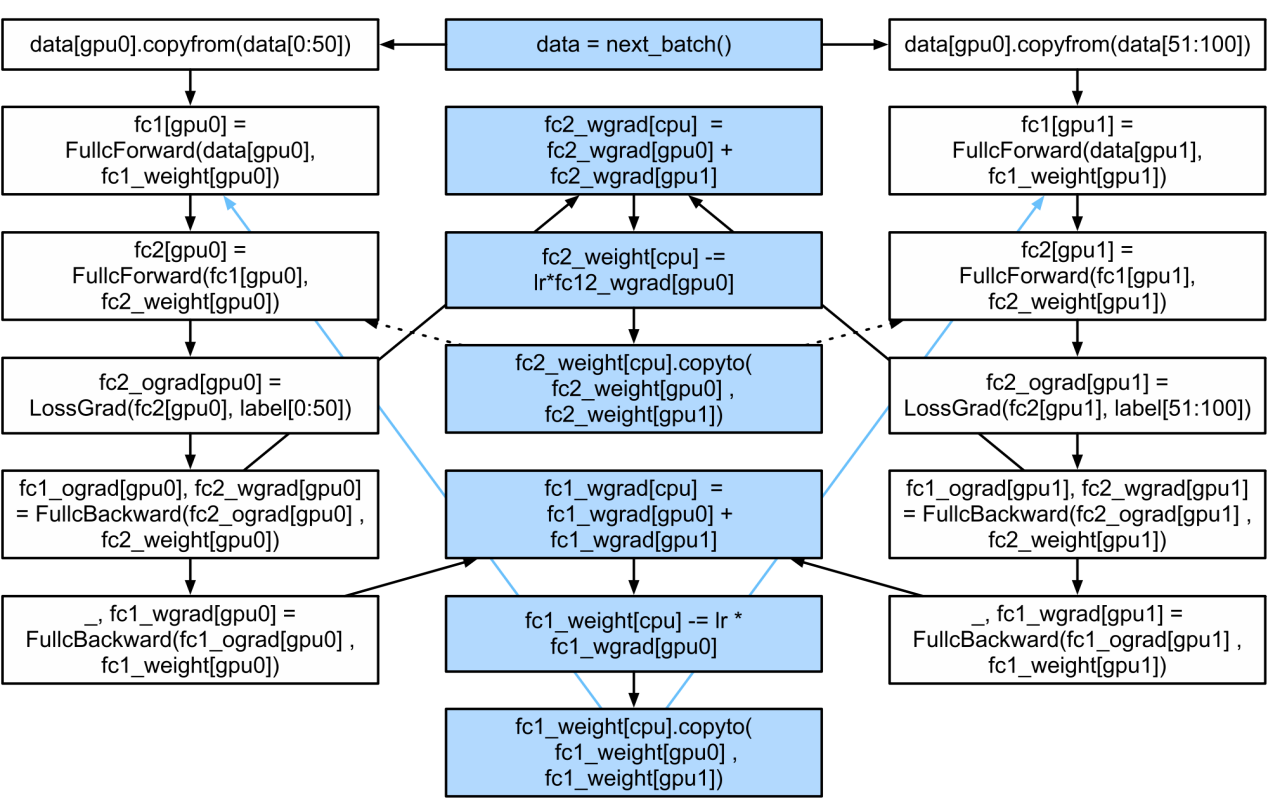
\includegraphics{images/image-0010.png}
\caption{CPU 与双 GPU 上两层 MLP 的计算依赖关系图}
\end{figure}

\hypertarget{ux53c2ux8003ux6587ux732e-33}{%
\subsection{参考文献}\label{ux53c2ux8003ux6587ux732e-33}}

\begin{itemize}
\tightlist
\item
  Aston Zhang, Zachary C. Lipton, Mu Li, Alexander J. Smola. (2023). \href{https://zh.d2l.ai/}{《动手学深度学习》}. Cambridge University Press.
\end{itemize}

\clearpage

\hypertarget{ux591agpuux8ba1ux7b97}{%
\section{多GPU计算}\label{ux591agpuux8ba1ux7b97}}

\hypertarget{ux4e00ux4e09ux79cdux62c6ux5206ux7b56ux7565}{%
\subsection{一、三种拆分策略}\label{ux4e00ux4e09ux79cdux62c6ux5206ux7b56ux7565}}

\begin{enumerate}
\def\labelenumi{\arabic{enumi}.}
\tightlist
\item
  网络拆分（拆分层/网络深度，纵向切分）（Pipeline Parallelism，PP）
\end{enumerate}

（1）原理：将神经网络的不同层分配给不同的GPU。例如，GPU 1处理第 1-10 层，GPU 2处理第11-20层。数据像流水线一样依次流过各个GPU。

（2）优点

能处理超大模型：因为模型的不同部分存在不同GPU上，单个GPU不需要存下整个模型，因此可以训练参数量巨大的模型。

（3）缺点

负载不均衡：层与层之间依赖性强，必须等待上一层计算完才能进行下一层，容易造成GPU空闲（等待），很难保证每一层的计算量恰好让每个GPU都忙碌且同步。

传输瓶颈：层与层之间的数据（激活值、梯度）传输量极大，可能超出GPU之间的带宽限制。

（4）结论：一般不推荐，只有在超大模型预训练中才会用上（和其他方法一起用），而不会用于前向推理（因为相同算力下，此方法最慢，会增加延迟，影响用户体验）。

\begin{enumerate}
\def\labelenumi{\arabic{enumi}.}
\setcounter{enumi}{1}
\tightlist
\item
  层内拆分（拆分通道/宽度，横向切分）（Tensor Parallelism，TP）
\end{enumerate}

（1）原理：将同一层内的计算工作拆分。如对于矩阵乘法Y = W*X，将权重矩阵W切成两半：W\_1和W\_2。GPU 1持有W\_1，计算一部分结果；GPU 2持有W\_2，计算另一部分结果。然后通过极高速的互联（NVLink）瞬间交换数据，把结果加起来，得到完整的token。又如，一个卷积层有k个通道，将其分给k个GPU，每个GPU负责一部分通道的计算。另外，层内拆分不仅是拆权重，长推理中KV Cache的K和V也会这样拆分。

（2）优点

显存线性扩展：显存占用被分摊，随着GPU数量增加，可以处理更宽、参数规模的网络。

性能提升：当权重规模大时，计算性能提升明显。

（3）缺点

极高的同步成本：由于每一层往往都会进行特征重组和交互（比如在卷积中就是通道重构），每一层计算结束都需要汇总所有GPU的结果才能进入下一层（屏障操作），导致大量等待。

通信开销大：需要传输的数据量可能比第一种方法还要大。

（4）结论：一般只用于大模型预训练和推理，单个GPU无法计算或无法在显存中存储全部权重，不得不拆分的情景。对于小模型，由于带宽成本和同步的复杂性，这种方法性价比低。

\begin{enumerate}
\def\labelenumi{\arabic{enumi}.}
\setcounter{enumi}{2}
\tightlist
\item
  数据并行（拆分数据）（Data Parallelism，DP）
\end{enumerate}

（1）原理

模型复制：每个GPU上都保留一份完整的模型参数副本。

数据拆分：将一个大批量（Batch）的数据切分成多个小份，分发给不同的GPU。比如完成100篇文章的掩码预测，每个GPU各自负责10篇（注：这时候GPU内部也是并行生成每篇的第一个词，然后每篇的第二个词，以此类推）；RLHF中，系统从Prompt库里拿出128个问题，GPU 1拿到问题 1-32，GPU 2拿到问题33-64，虽然 GPU 1必须按顺序生成第1个字、第2个字\ldots\ldots 但在同一毫秒内，GPU 1正在同时算它的32个句子的第T个字，GPU 2也是。

独立计算，统一更新：每个GPU独立计算自己那份数据的梯度，然后所有GPU的梯度进行聚合（求和或平均），最后用聚合后的梯度更新所有GPU上的模型参数。如上面RLHF的例子，只有当大家把句子都写完了，要开始算梯度更新模型的时候，才需要停下来互相交换信息。

（2）优点

实现简单：最容易落地，适用于几乎所有情况。

效率高：同步仅在处理完一个小批量后发生，且可以利用梯度计算的时间差进行部分通信掩盖。

吞吐量大：GPU越多，一次能处理的数据量（Batch Size）就越大，训练越快。

（3）缺点

受限于单卡显存：因为每个GPU都要存完整的模型，所以无法训练单卡显存装不下的超大模型。

（4）结论：最常用。随着现代GPU显存的增加，这是目前几乎所有模型在训练和推理中都会采用的方法。

（5）工作流程

分发数据：将一个随机的小批量数据（batch）均匀切分成k份。

局部计算：每个GPU拿着自己分到的数据，计算损失和梯度。

梯度聚合：将k个GPU算出的梯度收集起来进行合并。

梯度广播：将合并后的总梯度重新发回给每个GPU。

参数更新：每个GPU使用相同的总梯度更新自己维护的模型参数，确保所有GPU上的模型始终保持一致。

（6）实践中的关键调整

批量大小：在k个GPU上训练时，由于每个GPU的工作负载与单卡训练时一致，总的批量大小通常扩大k倍。

学习率：由于批量大小变大了，梯度的估计更准确了，通常需要相应地调大习率以加快收敛。

批量规范化：这是一个特例。因为BN依赖于批量的统计信息（均值和方差），直接在单卡上计算可能会因为单卡数据量小而不准确。通常需要调整，比如使用同步BN（SyncBN）或者为每个GPU保留独立的BN参数。

\hypertarget{ux4e8czerozero-redundancy-optimizer}{%
\subsection{二、ZeRO（Zero Redundancy Optimizer）}\label{ux4e8czerozero-redundancy-optimizer}}

这是目前大模型预训练用到的另一技术（DeepSpeed/FSDP核心）。

在标准的数据并行中，每张卡都存一份完整的模型，太浪费显存。ZeRO把模型参数``切开''，每个GPU存一小块。但和层内切分不同的是，TP中每个GPU分别计算``输入\emph{本GPU的参数''，计算完毕后再相加。ZeRO中，GPU 1会先向其他GPU借到所有需要的参数，再进行``输入}完整参数''的计算，算完马上扔掉不属于自己的（节省显存）。

TP 不仅仅是拆分了权重的\textbf{存储}，更重要的是它拆分了\textbf{计算过程}。它改变了矩阵乘法的数学执行方式。

\begin{itemize}
\tightlist
\item
  \textbf{场景}：我们要计算 \(Y = X \times W\)。矩阵 \(W\) 太大。
\item
  \textbf{做法}：

  \begin{itemize}
  \tightlist
  \item
    将 \(W\) 竖着切成两半：\(W_A\) 和 \(W_B\)。
  \item
    GPU 1 拿着 \(W_A\)，计算 \(Y_A = X \times W_A\)。
  \item
    GPU 2 拿着 \(W_B\)，计算 \(Y_B = X \times W_B\)。
  \end{itemize}
\item
  \textbf{关键点}：

  \begin{itemize}
  \tightlist
  \item
    \textbf{时刻都需要}：在计算这一层的整个过程中，GPU 1 和 GPU 2 都在干活。
  \item
    \textbf{通信极其频繁}：算完这一层，必须马上通过 NVLink 进行一次 \texttt{All-Reduce}（汇总），才能得到最终的 \(Y\) 去算下一层。
  \item
    \textbf{目的}：让单次矩阵计算变快，或者解决单卡算不动的问题。
  \end{itemize}
\end{itemize}

ZeRO 本质上还是\textbf{数据并行（Data Parallelism）}。这意味着，逻辑上每张 GPU 应该拥有一个\textbf{完整}的模型副本。但 ZeRO 说：``太浪费了，我们假装每个人都有完整的，但实际上每人只存一部分。''

\begin{itemize}
\tightlist
\item
  \textbf{场景}：我们在做数据并行。GPU 1 负责数据 A，GPU 2 负责数据 B。
\item
  \textbf{做法（以 ZeRO-3 为例）}：

  \begin{itemize}
  \tightlist
  \item
    参数 \(W\) 被切碎，GPU 1 存前半截，GPU 2 存后半截。\textbf{注意：这是静态存储时的状态。}
  \item
    \textbf{计算开始时（前向传播）}：

    \begin{enumerate}
    \def\labelenumi{\arabic{enumi}.}
    \tightlist
    \item
      \textbf{Broadcast（借参数）}：到了第 1 层，GPU 1 发现自己只有一半参数，它立刻向 GPU 2 要另一半。GPU 2 同理。
    \item
      \textbf{重组}：此时，GPU 1 和 GPU 2 的显存里都有了\textbf{完整的第 1 层参数}。
    \item
      \textbf{独立计算}：GPU 1 算自己的数据 A，GPU 2 算自己的数据 B。\textbf{注意：这里不是合力算一个矩阵，而是各算各的数据。}
    \item
      \textbf{丢弃}：算完第 1 层，为了省显存，大家把借来的参数马上删掉，只保留自己负责保管的那一小块。
    \end{enumerate}
  \end{itemize}
\item
  \textbf{关键点}：

  \begin{itemize}
  \tightlist
  \item
    \textbf{临时重组}：计算时，参数是完整的。
  \item
    \textbf{通信换显存}：用带宽（反复借参数、扔参数）来换取显存空间。
  \end{itemize}
\end{itemize}

一句话总结：TP 是把``干活''的任务拆分了（大家一起算）；ZeRO 是把``保管''的任务拆分了（大家轮流用）。

\hypertarget{ux4e09ux591aux79cdux65b9ux6cd5ux7684ux6df7ux5408ux4f7fux7528}{%
\subsection{三、多种方法的混合使用}\label{ux4e09ux591aux79cdux65b9ux6cd5ux7684ux6df7ux5408ux4f7fux7528}}

在训练大模型时，我们通常会混合使用多种方法：

\begin{enumerate}
\def\labelenumi{\arabic{enumi}.}
\item
  使用数据并行，根据batch划分数据；
\item
  用层内切分把模型切开（比如8张卡切分一个模型），为了让矩阵乘法能跑得动，且单层计算延迟低；
\item
  再在不同的机器节点之间使用ZeRO，如果不加ZeRO，每组TP在训练时都需要存一份完整的优化器状态（FP32格式的参数备份、动量、方差），其占显存是单纯模型参数的数倍；加了ZeRO，这些状态就可以打散存储在成百上千张卡上。
\item
  必要的时候使用层间切分。
\end{enumerate}

\hypertarget{ux53c2ux8003ux6587ux732e-34}{%
\subsection{参考文献}\label{ux53c2ux8003ux6587ux732e-34}}

\begin{itemize}
\tightlist
\item
  Aston Zhang, Zachary C. Lipton, Mu Li, Alexander J. Smola. (2023). \href{https://zh.d2l.ai/}{《动手学深度学习》}. Cambridge University Press.
\end{itemize}

\clearpage

\hypertarget{f1bux4e0edualpipe}{%
\section{1F1B与DualPipe}\label{f1bux4e0edualpipe}}

\hypertarget{ux4e00ux5206ux5e03ux5f0fux8badux7ec3ux6846ux67b6ux4e2dux7684ux57faux672cux8badux7ec3ux6b65ux9aa4}{%
\subsection{一、分布式训练框架中的基本训练步骤}\label{ux4e00ux5206ux5e03ux5f0fux8badux7ec3ux6846ux67b6ux4e2dux7684ux57faux672cux8badux7ec3ux6b65ux9aa4}}

\begin{enumerate}
\def\labelenumi{\arabic{enumi}.}
\tightlist
\item
  F（Forward）：前向计算
\end{enumerate}

动作：输入数据 \(x\) 经过当前层的算子（如矩阵乘法 \(Wx\)），输出激活值 \(y\)。

公式：

\[
y = f(x, \theta)
\]

关键任务：计算预测结果，并\textbf{缓存（Checkpointing）}中间层的激活值，留给后续反向传播使用。

在流水线并行中：F 的输出需要发送给下一个（Downstream）GPU 节点。

\begin{enumerate}
\def\labelenumi{\arabic{enumi}.}
\setcounter{enumi}{1}
\tightlist
\item
  B（Backward for Input / Activation Gradient）：激活梯度计算
\end{enumerate}

动作：根据上一层传回的梯度 \(\frac{\partial L}{\partial y}\)，计算对\textbf{当前层输入} \(x\) 的梯度。

公式：

\[
\nabla x = \frac{\partial L}{\partial x} = \frac{\partial L}{\partial y} \cdot \frac{\partial y}{\partial x}
\]

关键任务：它是反向传播的``接力棒''。计算出的 \(\nabla x\) 必须立刻传回给上一个（Upstream）GPU 节点，以便那一层继续计算。

地位：在流水线并行中，B 位于\textbf{关键路径（Critical Path）}上。如果 B 算得慢或传输延迟高，整个流水线都会卡住（产生 Bubble）。

\begin{enumerate}
\def\labelenumi{\arabic{enumi}.}
\setcounter{enumi}{2}
\tightlist
\item
  W（Backward for Weights / Parameter Gradient）：权重梯度计算
\end{enumerate}

动作：根据梯度 \(\frac{\partial L}{\partial y}\)，计算对\textbf{当前层参数} \(\theta\) 的梯度。

公式：

\[
\nabla \theta = \frac{\partial L}{\partial \theta} = \frac{\partial L}{\partial y} \cdot \frac{\partial y}{\partial \theta}
\]

关键任务：计算出的 \(\nabla \theta\) 会被存放在梯度缓冲区中，最终由优化器（Optimizer）用于更新模型权重。

地位：\(W\) \textbf{不在关键路径上}。因为 \(\nabla \theta\) 只需要在这一层本地更新，不需要传给其他 Rank 来解开计算依赖。

\hypertarget{ux4e8c1f1b}{%
\subsection{二、1F1B}\label{ux4e8c1f1b}}

假设我们有 4 个 GPU（Rank 0\textasciitilde3），流水线深度 \(PP = 4\)。

\begin{itemize}
\tightlist
\item
  \textbf{对于 Rank 0 来说}：它处理微批次 \(m_1\) 的前向计算（\(F_1\)）非常快。
\item
  \textbf{但是}：\(F_1\) 算完后，必须传给 Rank 1 \(\to\) Rank 2 \(\to\) Rank 3，在 Rank 3 算出 Loss 后，梯度再从 Rank 3 \(\to\) Rank 2 \(\to\) Rank 1，最后才传回 Rank 0。
\item
  \textbf{结论}：当 Rank 0 拿到 \(m_1\) 的梯度准备算反向（\(B_1\)）时，中间已经过去了一段很长的时间。
\end{itemize}

为了不让 GPU 闲着，Rank 0 在等待 \(B_1\) 的梯度传回来的这段时间里，会继续往后算 \(F_2, F_3, F_4, \dots\)。

\begin{itemize}
\tightlist
\item
  \(F_i\)：代表当前正在处理的第 \(i\) 个微批次的前向。
\item
  \(B_{i-k}\)：代表之前某个\textbf{已经跑完一圈回来}的微批次（第 \(i-k\) 个）的反向。
\end{itemize}

这里的 \(k\) 实际上取决于 GPU 所在的 Rank 位置。

\begin{itemize}
\tightlist
\item
  在流水线末端（如 Rank 3），\(F\) 和 \(B\) 靠得很近，\(k\) 很小。
\item
  在流水线顶端（如 Rank 0），\(F\) 和 \(B\) 隔得很远，\(k\) 很大。
\end{itemize}

``气泡''大小：

假设每个阶段（\(F\) 或 \(B\)）耗时为 1 个单位时间：

\begin{enumerate}
\def\labelenumi{\arabic{enumi}.}
\tightlist
\item
  \(T = 0\)：Rank 0 执行 \(F_1\)。
\item
  \(T = PP - 1\)：经过 \(PP - 1\) 跳，\(F_1\) 到达最后一个 Rank 并完成计算，立即算出 Loss。
\item
  \(T = PP\)：最后一个 Rank 开始执行反向计算 \(B_1\)。
\item
  \(T = PP + (PP - 1)\)：梯度经过 \(PP - 1\) 跳，传回 Rank 0。
\item
  \(T = 2PP - 1\)：Rank 0 终于可以开始执行 \(B_1\)。
\end{enumerate}

结论：在 Rank 0 看来，从 \(F_1\) 结束到 \(B_1\) 开始，中间隔了 \(2PP - 2\) 个时间片。

这里有一个概念上的区分：\textbf{单任务延迟} vs \textbf{流水线总气泡}。

\begin{itemize}
\tightlist
\item
  \textbf{总气泡（Bubble）}：指的是在整个训练任务中，所有 GPU 处于``空闲（Idle）''状态的总时间。
\item
  在 1F1B 中，Rank 0 在等待 \(B_1\) 回来的这段时间内，并没有闲着，而是在疯狂地跑 \(F_2, F_3, \dots, F_{PP}\)。
\item
  真正无法掩盖的空闲时间只有：最开始启动时的``热身''和最后结束时的``收尾''。将所有 GPU 的空闲时间相加再平均，每个 GPU 的平均气泡大小确实约为 \((PP - 1) \times (F + B)\)。
\end{itemize}

\hypertarget{ux4e09dualpipe}{%
\subsection{三、DualPipe}\label{ux4e09dualpipe}}

我们将以 \textbf{4 个 GPU（Rank 0-3）}、流水线并行深度 \(PP = 4\) 为例。

\begin{itemize}
\tightlist
\item
  \textbf{正向流（D1）}：数据从 \(R0 \to R1 \to R2 \to R3\)（逻辑层 L1 \(\to\) L8）。
\item
  \textbf{反向流（D2）}：数据从 \(R3 \to R2 \to R1 \to R0\)（逻辑层 L1 \(\to\) L8，注意是镜像的）。
\item
  \textbf{计算拆分}：每个阶段分为 \(F\)（前向）、\(B\)（算输入梯度，传给邻居）、\(W\)（算权重梯度，本地用）。
\end{itemize}

\hypertarget{ux4e00ux53ccux5411ux70edux8eabux9636ux6bb5}{%
\subsubsection{（一）双向热身阶段}\label{ux4e00ux53ccux5411ux70edux8eabux9636ux6bb5}}

\textbf{\(T1\)：双向同时启动}

\begin{itemize}
\tightlist
\item
  Rank 0：\(F_{D1}(m_1)\)
\item
  Rank 1：-
\item
  Rank 2：-
\item
  Rank 3：\(F_{D2}(n_1)\)
\end{itemize}

\textbf{\(T2\)：数据向中间汇聚}

\begin{itemize}
\tightlist
\item
  Rank 0：\(F_{D1}(m_2)\)
\item
  Rank 1：\(F_{D1}(m_1)\)
\item
  Rank 2：\(F_{D2}(n_1)\)
\item
  Rank 3：\(F_{D2}(n_2)\)
\end{itemize}

\textbf{\(T3\)：中间节点开始处理双向流}

\begin{itemize}
\tightlist
\item
  Rank 0：\(F_{D1}(m_3)\)
\item
  Rank 1：\(F_{D1}(m_2)+F_{D2}(n_1)\)
\item
  Rank 2：\(F_{D2}(n_2)+F_{D1}(m_1)\)
\item
  Rank 3：\(F_{D2}(n_3)\)
\end{itemize}

\textbf{\(T4\)：第一批双向流到达两端}

\begin{itemize}
\tightlist
\item
  Rank 0：\(F_{D1}(m_4)+F_{D2}(n_1)\)
\item
  Rank 1：\(F_{D1}(m_3)+F_{D2}(n_2)\)
\item
  Rank 2：\(F_{D2}(n_3)+F_{D1}(m_2)\)
\item
  Rank 3：\(F_{D2}(n_4)+F_{D1}(m_1)\)
\item
  备注：此时 \(m_1\) 到达 \(R3\)，\(n_1\) 到达 \(R0\)。
\end{itemize}

分析：在 \(T4\) 结束时，\(m_1\) 在 \(R3\) 算完了全部前向（逻辑 L1-L8），\(n_1\) 在 \(R0\) 算完了全部前向。从 \(T5\) 开始，系统将产生第一批梯度并进入复杂的对冲阶段。

注意：m1和n1是完全不同的数据批次。

\hypertarget{ux4e8cux7a33ux6001ux9636ux6bb5}{%
\subsubsection{（二）稳态阶段}\label{ux4e8cux7a33ux6001ux9636ux6bb5}}

在稳态下，一个 GPU 并不是按顺序执行，而是通过两个主要的\textbf{并行块（Candidate Blocks）}来工作。在一个完整的稳态步内，它包含以下两个核心对冲：

\textbf{对冲 A：\(F_{D1}\) 与 \(B_{D2}\) 的完全重叠}

\begin{itemize}
\tightlist
\item
  \textbf{计算内容}：GPU 同时启动两个算子：

  \begin{enumerate}
  \def\labelenumi{\arabic{enumi}.}
  \tightlist
  \item
    正向流新批次的前向计算 \(F_{D1}(m_i)\)。
  \item
    反向流老批次的激活梯度计算 \(B_{D2}(n_j)\)。
  \end{enumerate}
\item
  \textbf{通信掩盖}：

  \begin{itemize}
  \tightlist
  \item
    在计算 \(F_{D1}\) 时，后台接收 \(B_{D2}\) 需要的下游梯度。
  \item
    在计算 \(B_{D2}\) 时，后台发送 \(F_{D1}\) 产生的激活值。
  \end{itemize}
\item
  \textbf{结论}：只要计算时间 \(T(F) \approx T(B)\)，这两个算子就能把彼此的通信时间完全吞掉。
\end{itemize}

\textbf{对冲 B：\(F_{D2}\) 与 \(B_{D1}\) 的完全重叠}

\begin{itemize}
\tightlist
\item
  与上述逻辑镜像，处理反向流的前向和正向流的激活梯度。
\end{itemize}

\textbf{步骤 C：填补 \(W\)（Weight Gradient）}

\begin{itemize}
\tightlist
\item
  \textbf{计算}：上述 \(B\) 计算完成后，立即在后台异步算 \(W\)（权重梯度）。
\item
  \textbf{原理}：\(W\) 不影响任何人，它是``计算废料''，哪里有缝隙就塞在哪里。
\end{itemize}

在一个对冲周期（如 \(F_{D1}\) 与 \(B_{D2}\) 对冲）内共有4个通信步骤，都被掩盖在计算时间中：

在 \(F_{D1}\) 计算时：

\begin{itemize}
\item
  \texttt{Send-Backward-D2}：把上一批次算好的 \(n_{j-1}\) 梯度发给右边。
\item
  \texttt{Recv-Backward-D2}：从左边接收本批次 \(n_j\) 的梯度。
\end{itemize}

在 \(B_{D2}\) 计算时：

\begin{itemize}
\item
  \texttt{Send-Forward-D1}：把算好的 \(m_i\) 激活值发给右边。
\item
  \texttt{Recv-Forward-D1}：从左边接收下一批次 \(m_{i+1}\) 的激活值。
\end{itemize}

\hypertarget{ux4e09ux6536ux5c3eux9636ux6bb5}{%
\subsubsection{（三）收尾阶段}\label{ux4e09ux6536ux5c3eux9636ux6bb5}}

当所有微批次的前向都跑完了，GPU 进入纯反向模式。

\begin{enumerate}
\def\labelenumi{\arabic{enumi}.}
\tightlist
\item
  \textbf{处理剩余的 \(B\)}：把最后几个微批次的输入梯度算完并传走。此时已经没有 \(F\) 可以对冲了，但因为 \(PP\) 被分成了两个方向，气泡的绝对时长减半。
\item
  \textbf{全力算 \(W\)}：这是最后的体力活，所有 GPU 并行计算自己负责的层权重更新。
\end{enumerate}

\hypertarget{ux56dbux6c14ux6ce1ux51cfux5c11ux7684ux6838ux5fc3ux539fux56e0}{%
\subsubsection{（四）气泡减少的核心原因}\label{ux56dbux6c14ux6ce1ux51cfux5c11ux7684ux6838ux5fc3ux539fux56e0}}

在 1F1B 中，Rank 0 算出 \(F_1\) 后，要等 \(2(PP - 1)\) 个时间片才能拿到梯度算 \(B_1\)。

\[
T_{\mathrm{wait}} = (PP - 1) \times (F + B)
\]

DualPipe采取了以下方式：

\begin{enumerate}
\def\labelenumi{\arabic{enumi}.}
\tightlist
\item
  \textbf{双向对冲（Bidirectional）}：

  \begin{itemize}
  \tightlist
  \item
    在 1F1B 等待梯度的时间里，DualPipe 让 GPU 去跑``另一个方向''的前向和反向。
  \item
    \textbf{数学逻辑}：将一个 PP 链拆成两个半深度的 PP 链对冲。气泡从 \((PP - 1)\) 变成了 \(\left(\frac{PP}{2} - 1\right)\)。
  \end{itemize}
\item
  \textbf{\(B\) 与 \(W\) 拆分（Zero Bubble 思想）}：

  \begin{itemize}
  \tightlist
  \item
    在传统做法中，反向传播是 \(B + W\)。必须等这两个都算完，梯度才能发给上一个 GPU。
  \item
    DualPipe 算完 \(B\)（只需矩阵乘法的一半工作量）\textbf{立即就把梯度发走}。这样邻居 GPU 就能提前开始干活。
  \item
    \textbf{结果}：关键路径上的等待时间进一步压缩。
  \end{itemize}
\item
  \textbf{完全重叠（Full Overlap）}：

  \begin{itemize}
  \tightlist
  \item
    利用现代 GPU 的双工带宽（NVLink 可以同时全速 Send 和 Recv）。
  \item
    DualPipe 调度算法保证了：\textbf{当 GPU 在做计算时，带宽始终是满的；当带宽在传输时，SM 核心始终在计算。}
  \end{itemize}
\end{enumerate}

\hypertarget{ux4e94ux6298ux53e0ux6d41ux6c34ux7ebfux6280ux672f}{%
\subsubsection{（五）折叠流水线技术}\label{ux4e94ux6298ux53e0ux6d41ux6c34ux7ebfux6280ux672f}}

DualPipe的``代价''是一个GPU需要存两倍的权重。原因：

\begin{quote}
正向流 Direction 1：从 \(Rank_0 \rightarrow Rank_3\)。Rank 0 必须有第 1 层。

反向流 Direction 2：从 \(Rank_3 \rightarrow Rank_0\)。但请注意，反向流也是一个完整的前向-反向过程。如果它从 Rank 3 开始起步，Rank 3 就必须有第 1 层。

这样一来，第 1 层在 Rank 0 和 Rank 3 都有，参数量自然翻倍了。
为了解决这个问题，可以采用``折叠''的方法：
\end{quote}

在折叠架构下，我们不再让 Rank 0 和 Rank 3 都存第 1 层，而是这样分配 Stage：

\begin{longtable}[]{@{}lll@{}}
\toprule
物理 Rank & 负责的逻辑 Stage（1x 参数，不冗余） & 物理位置属性 \\
\midrule
\endhead
Rank 0 & Stage 0（入口）和 Stage 7（出口） & 流水线两头 \\
Rank 1 & Stage 1 和 Stage 6 & \\
Rank 2 & Stage 2 和 Stage 5 & \\
Rank 3 & Stage 3 和 Stage 4 & 流水线折返点 \\
\bottomrule
\end{longtable}

虽然每个 Stage 只存了一份（1x 参数），但因为每个 GPU 现在都手握一个靠前的 Stage（如 S0）和一个靠后的 Stage（如 S7），对冲依然可以发生：

\begin{enumerate}
\def\labelenumi{\arabic{enumi}.}
\tightlist
\item
  任务组合：当 Rank 0 正在处理微批次 \(m_{10}\) 的 Stage 0（前向计算）时，它手里可能正好拿着微批次 \(m_1\) 绕了一圈回来的 Stage 7（前向或反向计算）。
\item
  算子对冲：

  \begin{itemize}
  \tightlist
  \item
    计算 A：\(F_{S_0}\)（新批次的前向）。
  \item
    计算 B：\(B_{S_7}\)（老批次的反向）。
  \end{itemize}
\item
  通信掩盖：

  \begin{itemize}
  \tightlist
  \item
    Rank 0 在发送 \(F_{S_0}\) 给 Rank 1 的同时，正好在接收 Rank 1 传回来的 \(B_{S_7}\) 梯度。
  \end{itemize}
\end{enumerate}

这就是``折叠''的精髓：它利用了流水线的深度（一个微批次从 S0 到 S7 走一圈很慢）创造了时间差，让同一个 GPU 在同一时间处理不同生命周期的任务。
但实际上很多大模型并不一定会用``折叠''的方法，原因有两方面。

\begin{enumerate}
\def\labelenumi{\arabic{enumi}.}
\tightlist
\item
  MoE模型的特点
\end{enumerate}

在一个超大规模 MoE 模型中，模型参数被分为两部分：

\begin{itemize}
\tightlist
\item
  \textbf{共享参数（Shared Parameters）}：包括注意力机制（Attention）、层归一化（LayerNorm）和一些共享的稠密层。
\item
  \textbf{专家参数（Expert Parameters）}：MoE 层中成百上千个独立的专家（MLP 块）。
\end{itemize}

这是最核心的工程实现细节：\textbf{专家参数是不参与流水线镜像冗余的。}

在分布式训练中，我们通常同时使用 PP（Pipeline Parallelism）和 EP（Expert Parallelism）：

\begin{enumerate}
\def\labelenumi{\arabic{enumi}.}
\tightlist
\item
  \textbf{PP 决定了路径}：它决定了微批次在哪几个 GPU 之间流转。
\item
  \textbf{EP 决定了存放}：它决定了某一个具体的专家 \(E_{100}\) 物理上存在在哪块显存里。
\end{enumerate}

在 DualPipe 的双向流中：

\begin{itemize}
\tightlist
\item
  当一个微批次运行到某一层需要调用专家时，它会发起一个 All-to-All 通信，去寻找那个专家所在的物理 GPU。
\item
  无论这个微批次是属于``正向流''还是``反向流''，它去寻找的都是同一个物理地址上的专家。
\item
  \textbf{结论：}专家参数在整个集群里依然只存了一份。DualPipe 只需要在每个 Rank 上多存一份轻量级的共享层参数和路由逻辑（Router）即可。
\end{itemize}

\begin{enumerate}
\def\labelenumi{\arabic{enumi}.}
\setcounter{enumi}{1}
\tightlist
\item
  激活值对显存占用更大
\end{enumerate}

对于超长上下文（Context Length）训练，显存瓶颈往往不是参数（Weights），而是激活值。

\begin{itemize}
\tightlist
\item
  在训练时，为了反向传播，每一层的前向计算结果都要存下来。
\item
  DualPipe 的显存压力：真正让显存紧张的是它同时在跑两个方向的流，这意味着显存里要同时存放 \(m\) 批次和 \(n\) 批次的激活值。
\end{itemize}

但 DeepSeek 巧妙地化解了这一点：

\begin{itemize}
\tightlist
\item
  通过 MLA（Multi-head Latent Attention）大幅压缩了 KV Cache 和激活值的体积。
\item
  配合 Recomputation（激活值重计算）技术，可以在需要时再计算部分激活值，用计算时间换取显存空间。
\item
  相比之下，多存那一套共享参数所占用的几 GB 显存，简直是``洒洒水''。
\end{itemize}

\begin{enumerate}
\def\labelenumi{\arabic{enumi}.}
\setcounter{enumi}{2}
\tightlist
\item
  训练调度方面
\end{enumerate}

带宽压榨：

1x 参数的折叠流水线在调度上非常死板（必须走 V 字型）。而 2x 参数的 DualPipe 拥有两条完全独立且对称的路径，这使得它能百分之百跑满双向 NVLink 带宽，调度灵活性极高。

气泡率的极致追求：

在折叠模型中，由于 \(B\) 和 \(W\) 的依赖关系更复杂，很难做到像 DualPipe 那样几乎``零气泡''。DeepSeek 的目标是把 MFU（模型算力利用率）推向 70\% 以上，2x 冗余是一笔划算的交易。

\hypertarget{ux53c2ux8003ux6587ux732e-35}{%
\subsection{参考文献}\label{ux53c2ux8003ux6587ux732e-35}}

\begin{itemize}
\tightlist
\item
  Narayanan, D., Harlap, A., Phanishayee, A., et al.~(2019). \href{https://dl.acm.org/doi/10.1145/3341301.3359646}{PipeDream: Generalized Pipeline Parallelism for DNN Training}. SOSP 2019.
\item
  DeepSeek-AI. (2024). \href{https://arxiv.org/abs/2412.19437}{DeepSeek-V3 Technical Report}. arXiv:2412.19437.
\end{itemize}

\clearpage
